\documentclass{article}
% Change "article" to "report" to get rid of page number on title page
\usepackage{amsmath,amsfonts,amsthm,amssymb}
\usepackage{setspace}
\usepackage{Tabbing}
\usepackage{fancyhdr}
\usepackage{enumerate,lastpage}
\usepackage{extramarks}
\usepackage{chngpage}
\usepackage{soul,color,alltt}
\usepackage{graphicx,float,wrapfig}
\usepackage{multirow,comment}

% In case you need to adjust margins:
\topmargin=-0.45in      %
\evensidemargin=0in     %
\oddsidemargin=0in      %
\textwidth=6.5in        %
\textheight=9.0in       %
\headsep=0.25in         %

% Homework Specific Information
\newcommand{\hmwkTitle}{Lane Assignment}
\newcommand{\hmwkClass}{}
\newcommand{\hmwkAuthorName}{Donglai\ Wei}


% Setup the header and footer
\pagestyle{fancy}                                                       %
\lhead{\hmwkAuthorName}                                                 %
\rhead{\firstxmark}                                                     %
\lfoot{\lastxmark}                                                      %
\cfoot{}                                                                %
\rfoot{Page\ \thepage\ of\ \pageref{LastPage}}                          %
\renewcommand\headrulewidth{0.4pt}                                      %
\renewcommand\footrulewidth{0.4pt}                                      %

% This is used to trace down (pin point) problems
% in latexing a document:
%\tracingall

%%%%%%%%%%%%%%%%%%%%%%%%%%%%%%%%%%%%%%%%%%%%%%%%%%%%%%%%\begin{enumerate}

% Some tools
\newcommand{\enterProblemHeader}[1]{\nobreak\extramarks{#1}{#1 continued on next page\ldots}\nobreak%
                                    \nobreak\extramarks{#1 (continued)}{#1 continued on next page\ldots}\nobreak}%
\newcommand{\exitProblemHeader}[1]{\nobreak\extramarks{#1 (continued)}{#1 continued on next page\ldots}\nobreak%
                                   \nobreak\extramarks{#1}{}\nobreak}%

\newlength{\labelLength}
\newcommand{\labelAnswer}[2]
  {\settowidth{\labelLength}{#1}%
   \addtolength{\labelLength}{0.25in}%
   \changetext{}{-\labelLength}{}{}{}%
   \noindent\fbox{\begin{minipage}[c]{\columnwidth}#2\end{minipage}}%
   \marginpar{\fbox{#1}}%

   % We put the blank space above in order to make sure this
   % \marginpar gets correctly placed.
   \changetext{}{+\labelLength}{}{}{}}%

\setcounter{secnumdepth}{0}
\newcommand{\homeworkProblemName}{}%
\newcounter{homeworkProblemCounter}%
\newenvironment{homeworkProblem}[1][Problem \arabic{homeworkProblemCounter}]%
  {\stepcounter{homeworkProblemCounter}%
   \renewcommand{\homeworkProblemName}{#1}%
   \section{\homeworkProblemName}%
   \enterProblemHeader{\homeworkProblemName}}%
  {\exitProblemHeader{\homeworkProblemName}}%

\newcommand{\problemAnswer}[1]
  {\noindent\fbox{\begin{minipage}[c]{\columnwidth}#1\end{minipage}}}%

\newcommand{\problemLAnswer}[1]
  {\labelAnswer{\homeworkProblemName}{#1}}

\newcommand{\homeworkSectionName}{}%
\newlength{\homeworkSectionLabelLength}{}%
\newenvironment{homeworkSection}[1]%
  {% We put this space here to make sure we're not connected to the above.
   % Otherwise the changetext can do funny things to the other margin

   \renewcommand{\homeworkSectionName}{#1}%
   \settowidth{\homeworkSectionLabelLength}{\homeworkSectionName}%
   \addtolength{\homeworkSectionLabelLength}{0.25in}%
   \changetext{}{-\homeworkSectionLabelLength}{}{}{}%
   \subsection{\homeworkSectionName}%
   \enterProblemHeader{\homeworkProblemName\ [\homeworkSectionName]}}%
  {\enterProblemHeader{\homeworkProblemName}%

   % We put the blank space above in order to make sure this margin
   % change doesn't happen too soon (otherwise \sectionAnswer's can
   % get ugly about their \marginpar placement.
   \changetext{}{+\homeworkSectionLabelLength}{}{}{}}%

\newcommand{\sectionAnswer}[1]
  {% We put this space here to make sure we're disconnected from the previous
   % passage

   \noindent\fbox{\begin{minipage}[c]{\columnwidth}#1\end{minipage}}%
   \enterProblemHeader{\homeworkProblemName}\exitProblemHeader{\homeworkProblemName}%
   \marginpar{\fbox{\homeworkSectionName}}%

   % We put the blank space above in order to make sure this
   % \marginpar gets correctly placed.
   }%

%%%%%%%%%%%%%%%%%%%%%%%%%%%%%%%%%%%%%%%%%%%%%%%%%%%%%%%%%%%%%



%%%%%%%%%%%%%%%%%%%%%%%%%%%%%%%%%%%%%%%%%%%%%%%%%%%%%%%%%%%%%
% Make title
\title{\vspace{0.3in}\textmd{\textbf{\hmwkTitle}}}
\date{2011.11.13}
%%%%%%%%%%%%%%%%%%%%%%%%%%%%%%%%%%%%%%%%%%%%%%%%%%%%%%%%%%%%%

\begin{document}
\begin{spacing}{1.1}
\maketitle

\section{0. Intro}
Obseration of shared road segments: how to model it?
\begin{figure}
\centering
\begin{tabular}{cc}
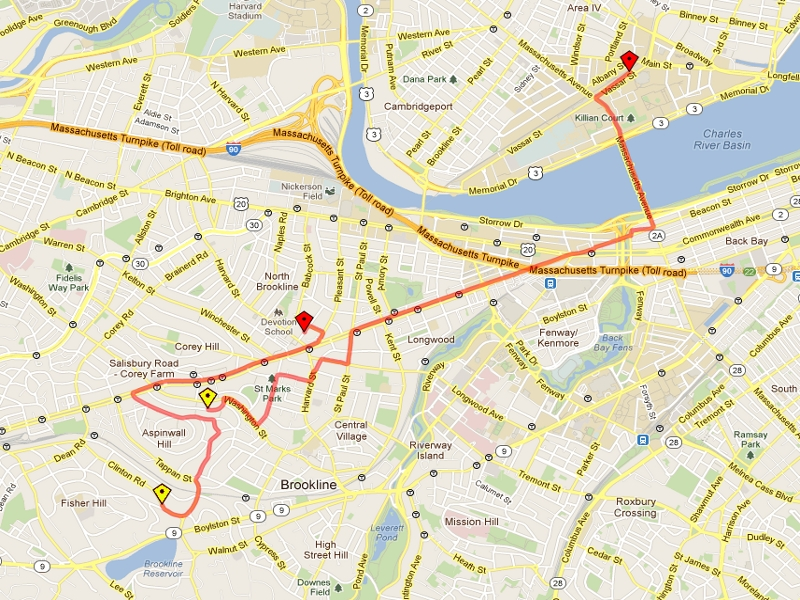
\includegraphics[width=3in,height=2in]{day1.jpg} &
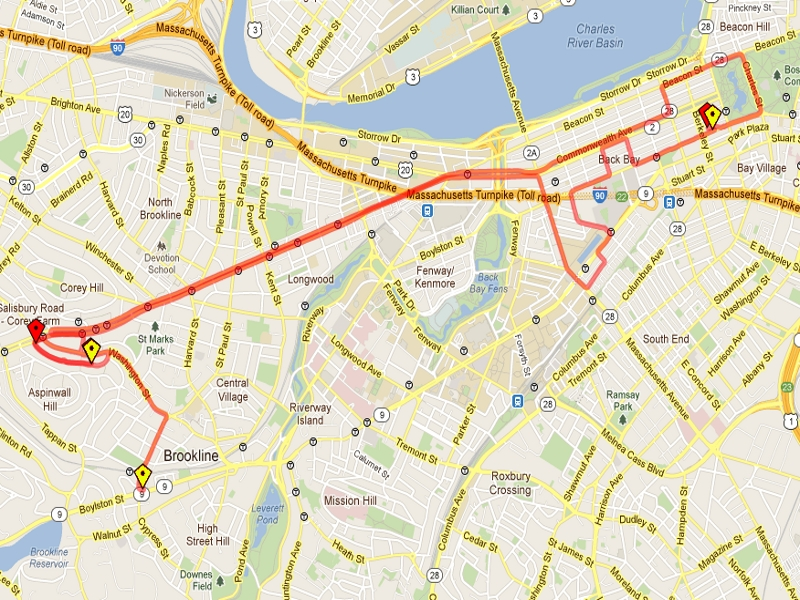
\includegraphics[width=3in,height=2in]{day2.jpg}
\end{tabular}
\begin{tabular}{cc}
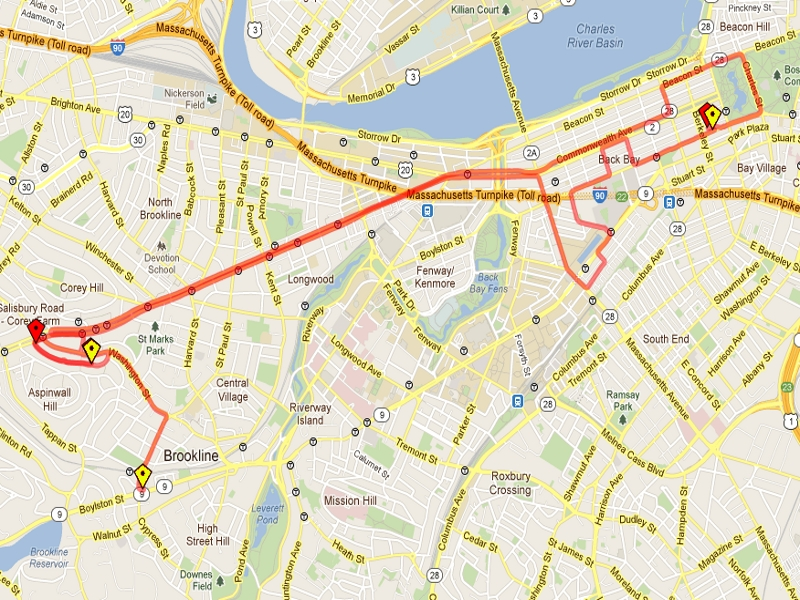
\includegraphics[width=3in,height=2in]{day3.jpg} &
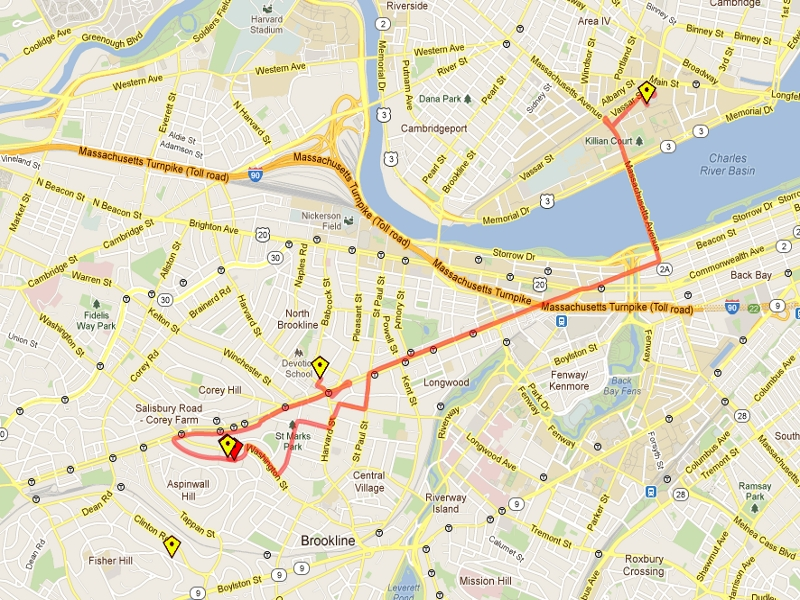
\includegraphics[width=3in,height=2in]{day4.jpg}
\end{tabular}
\caption{Beacon ST}
\end{figure}

\begin{figure}
\caption{15 routes}
  \centering
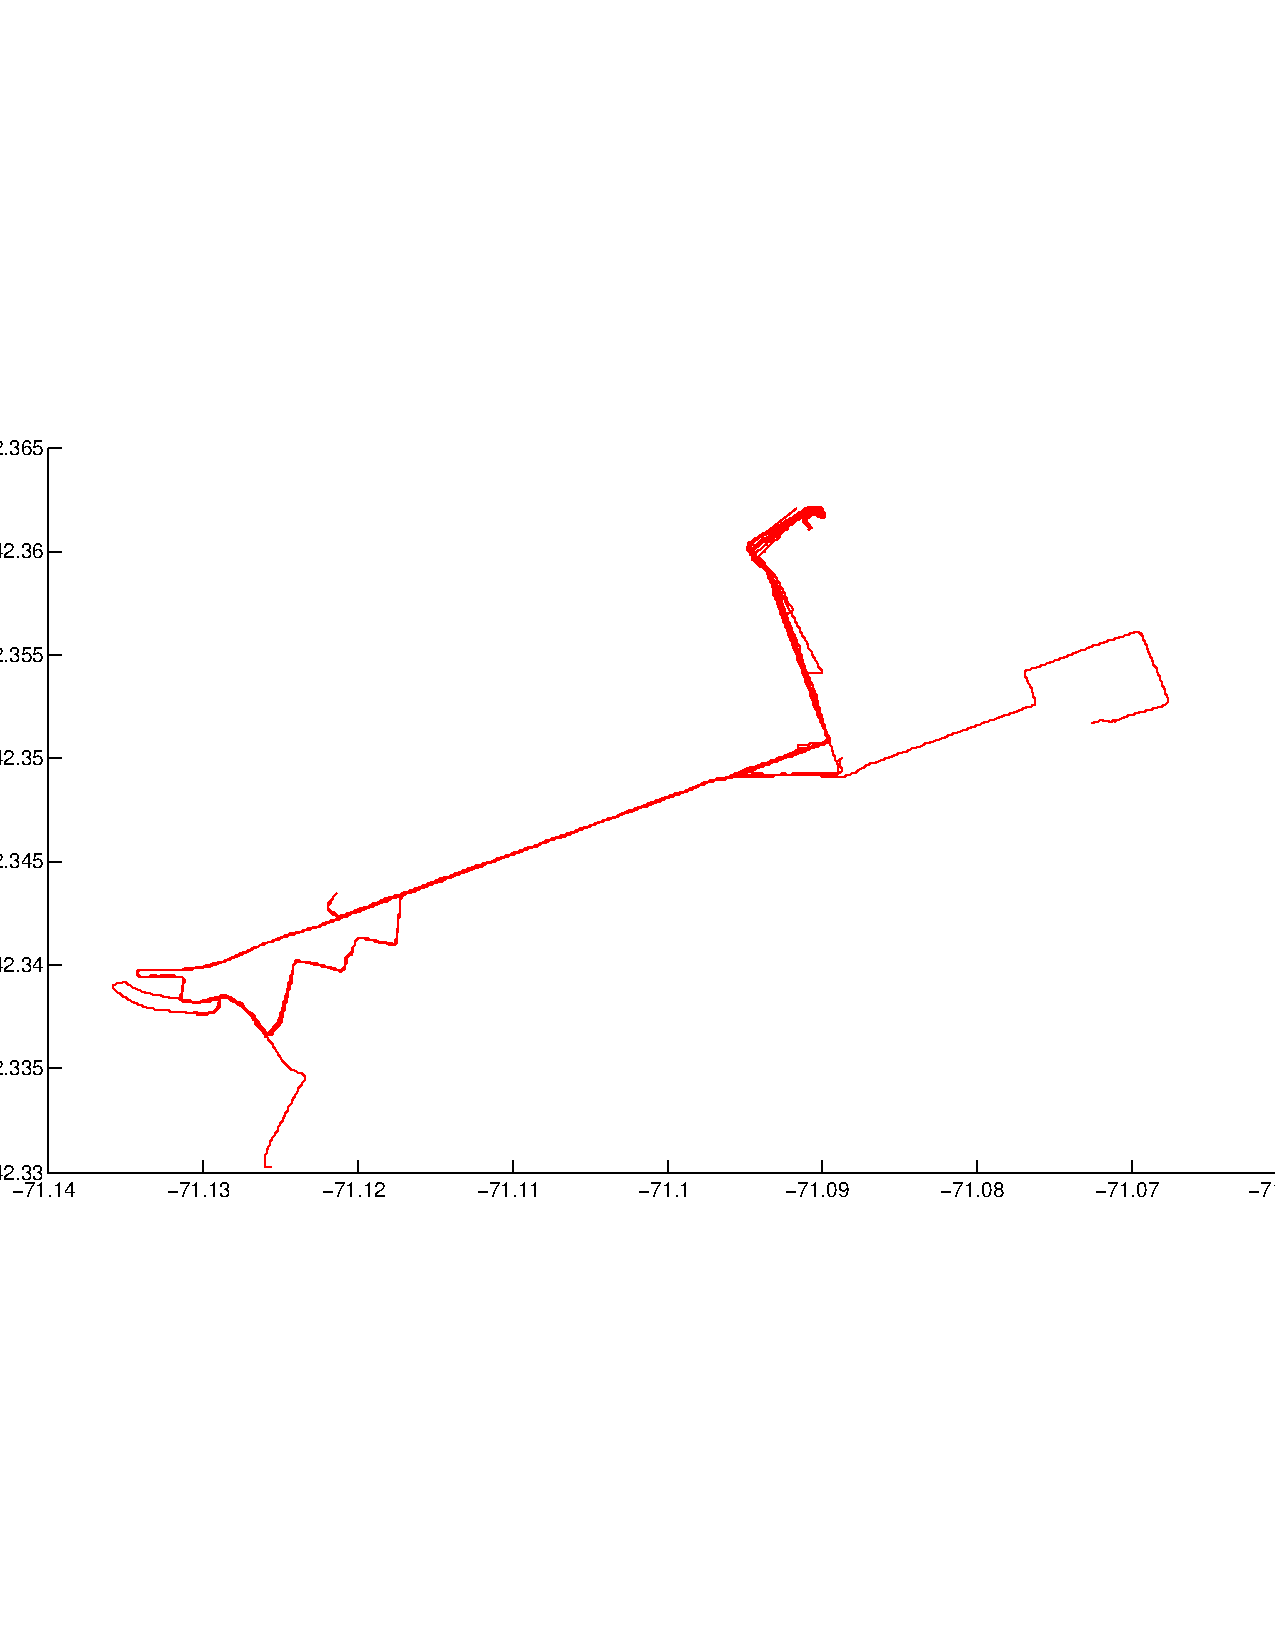
\includegraphics[width=3in,height=4in]{routes.pdf}
\end{figure}

\newpage
\section{1. Independent Mixture of Gaussian}
{\bf Model:}\\
x=(lat,lon)$|z_x$ $\sim \sum\limits_{k=1}^{K}\delta(z_x=k)\mathcal{N}(\mu_k,\Sigma_{k})$\\
where:\\
$z_x$ is the road segment assignment of x, \\
{\bf Algo:}\\
EM\\\\
\begin{figure}[h]
\caption{independent MoG model}
  \centering
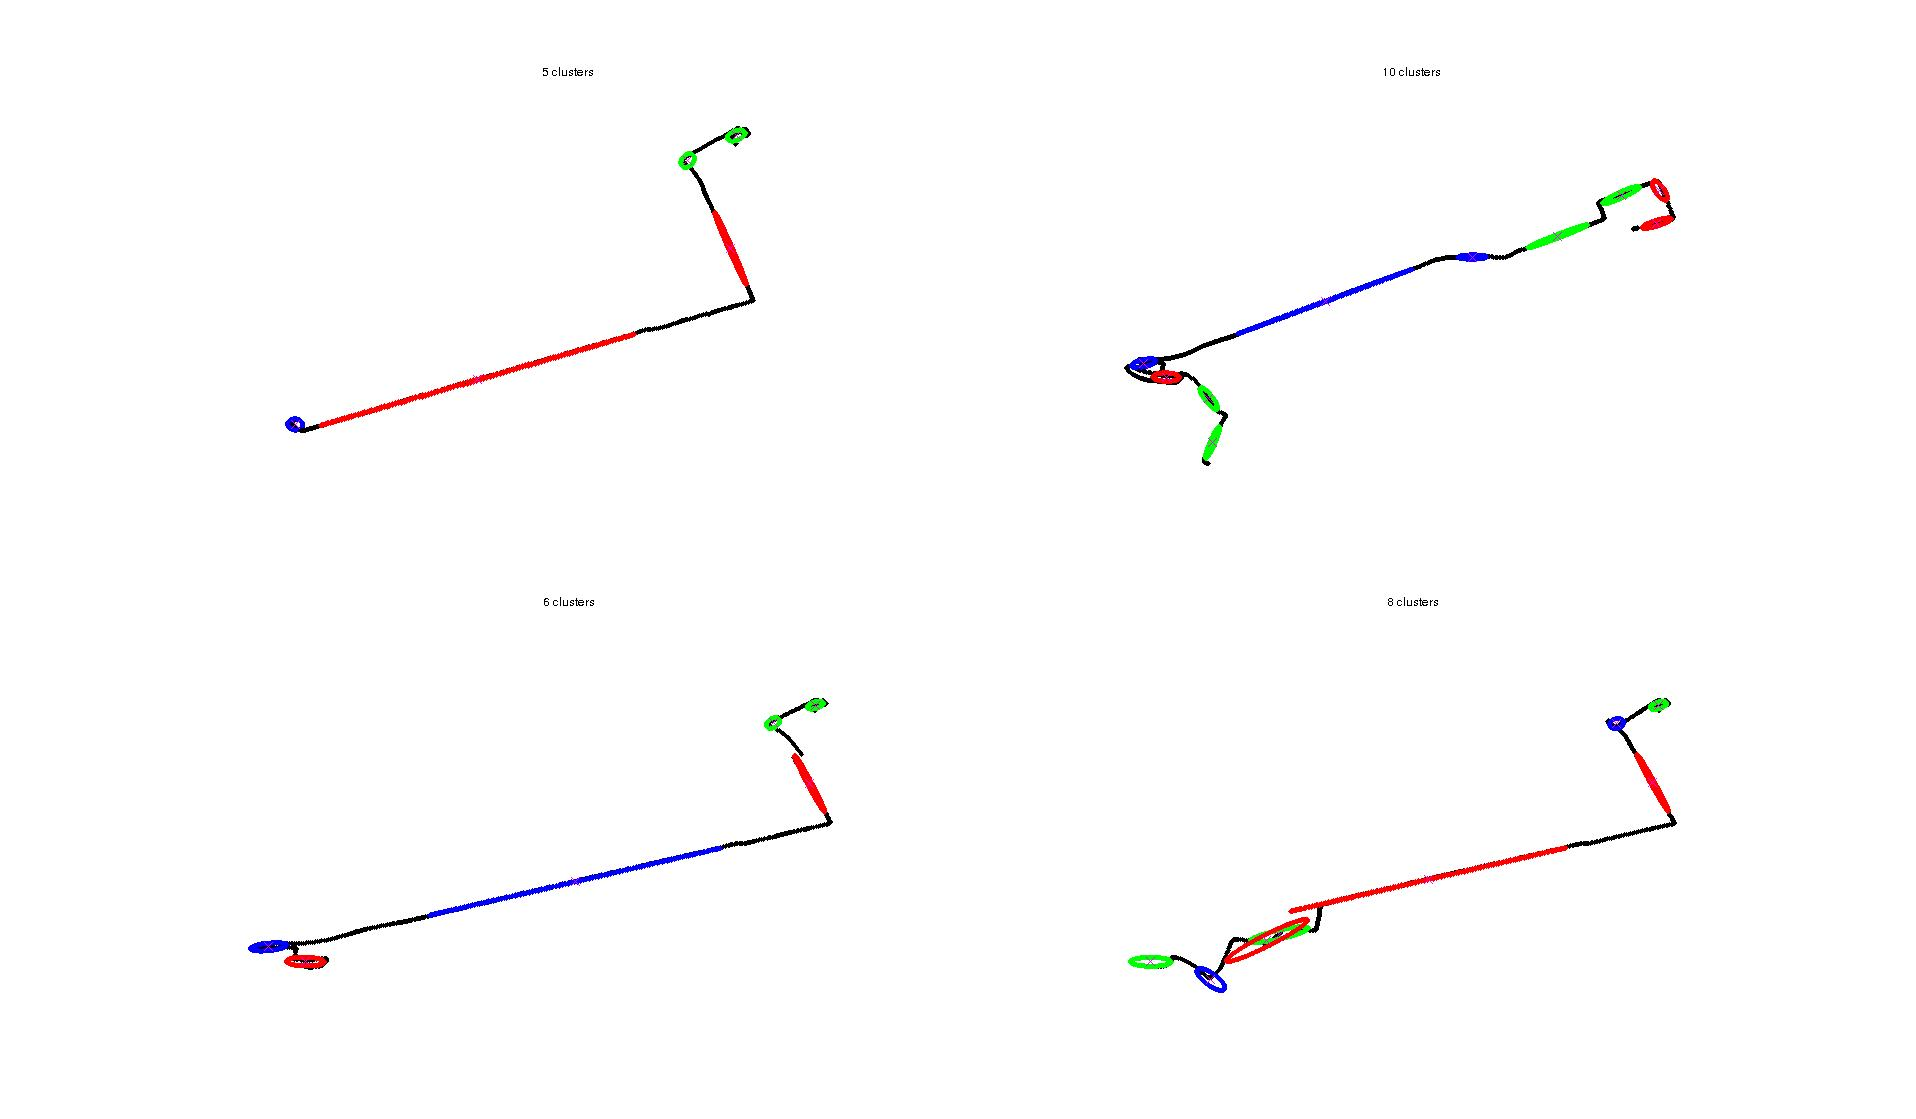
\includegraphics[width=3in,height=4in]{ind_cluster.jpg}
\end{figure}


\newpage
\section{2) Mixture of Gaussian with shared prior}
\subsection{2.1) Graphical Model:}
\begin{figure}[h]
\caption{Graphical Model}
  \centering
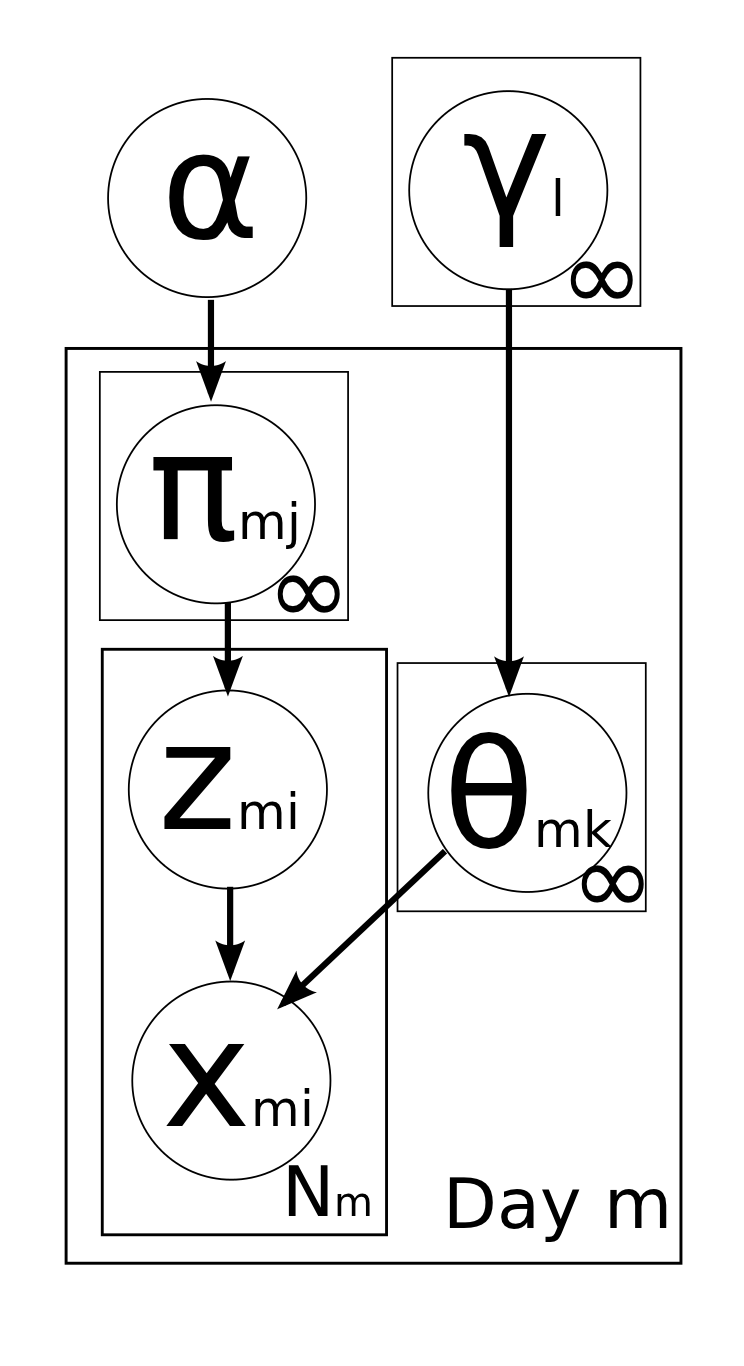
\includegraphics[width=3in,height=4in]{gm.png}
\end{figure}
$
\theta_{mk}:(\mu_{mk},\sigma_{mk})\\
\gamma_{l}:(\mu_{l},\mbox{Inv-Wishart}(l))\\
\pi_{mj}| \alpha \sim GEM(\alpha)\\
z_{mi}|\{\pi_{j}\}_{j=1}^{\infty}}\sim \pi_{z_{mi}}\\
x_{t}|\{\theta_{mk}\}_{k=1}^{\infty},z_{mi}\sim \mathcal{N}(\mu_{z_{mi}},\Sigma_{z_{mi}})\\
\Sigma_{mk}\sim \mbox{Inv-Wishart}(k))\\
\mu_{mk}\sim  \mathcal{N}(k))$\\
{\bf Algo:}\\
Meanfield \\\\
\newpage
\subsection{2.2) Result}
\subsubsection{2.2.1) Shared topics}
\begin{figure}[h]
\caption{Comparison Result}
  \centering
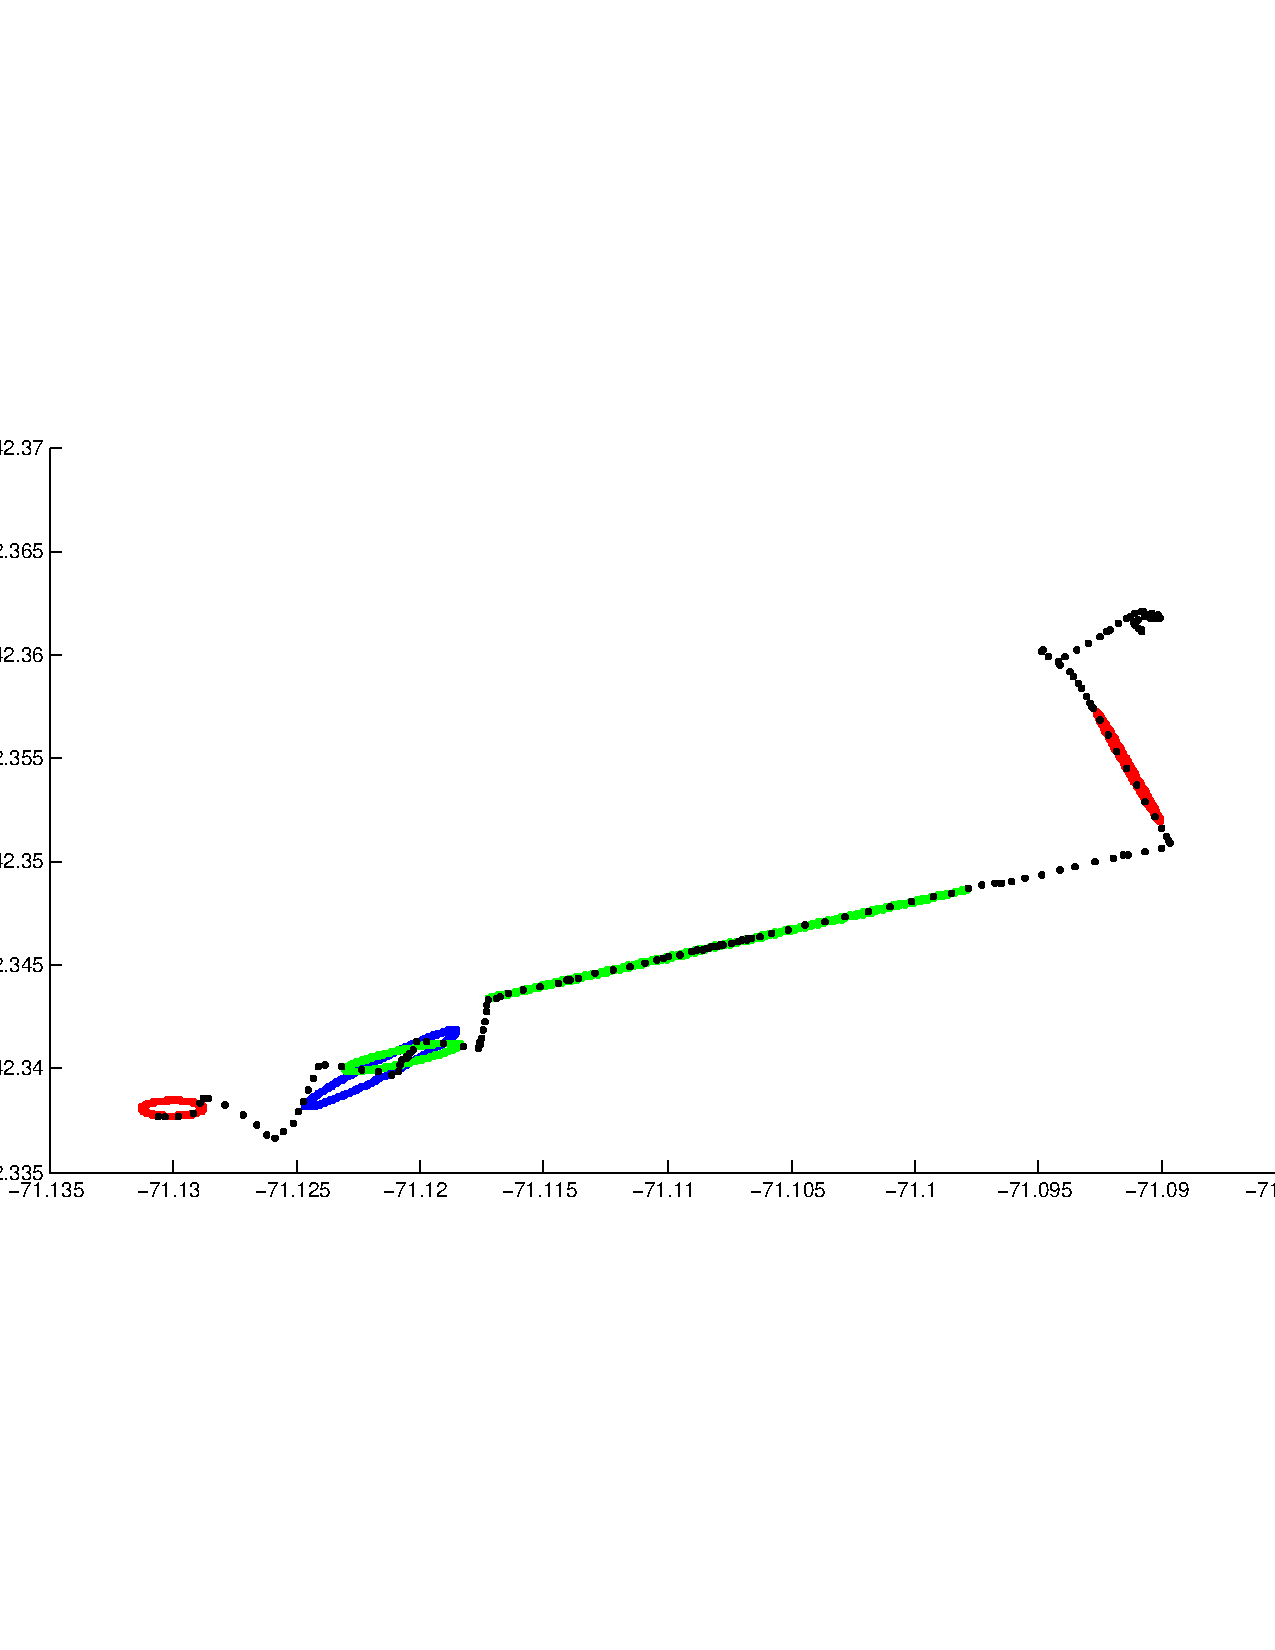
\includegraphics[width=5in,height=4in]{topics.pdf}\\
\end{figure}
\subsubsection{2.2.2) Rate of KL divergence}
\begin{figure}[h]
\caption{Comparison Result}
  \centering
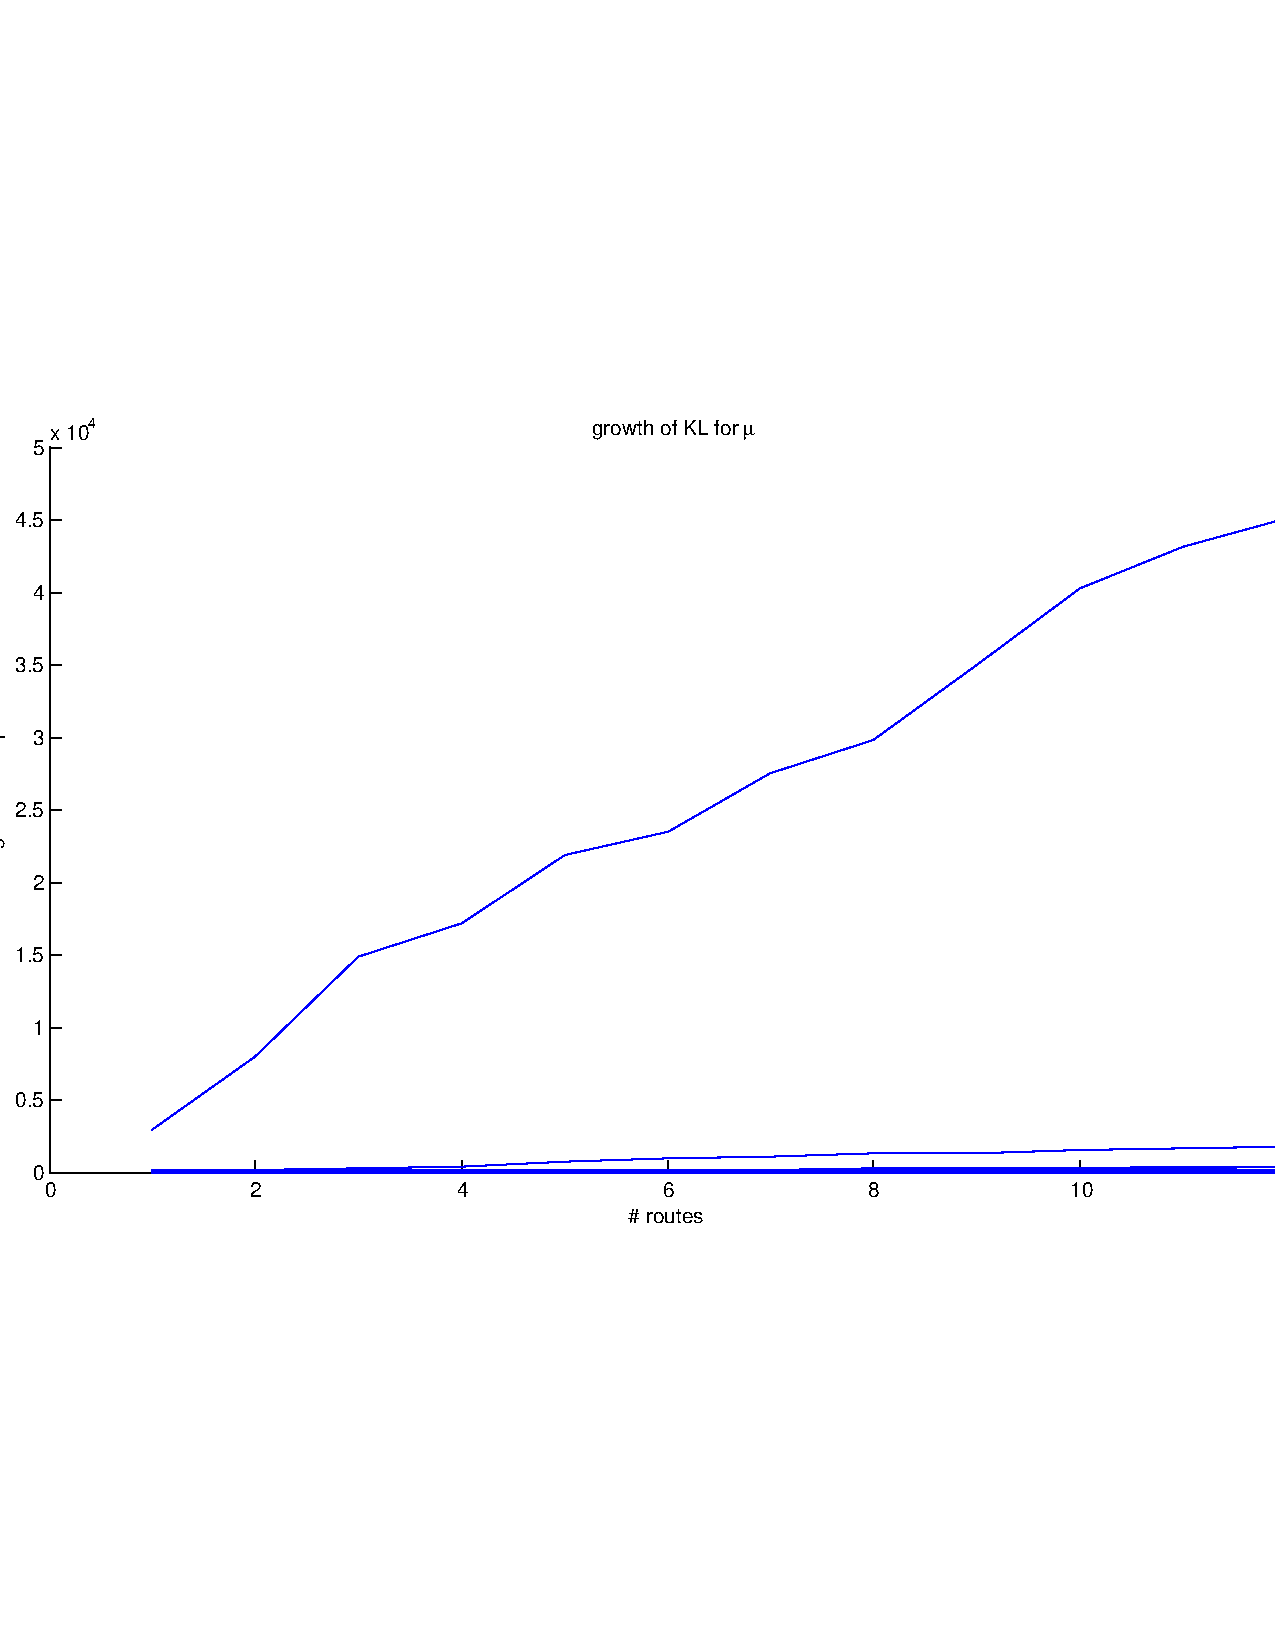
\includegraphics[width=5in,height=4in]{kl.pdf}\\
\end{figure}

\end{spacing}
\end{document}

%%%%%%%%%%%%%%%%%%%%%%%%%%%%%%%%%%%%%%%%%%%%%%%%%%%%%%%%%%%%%
